\section{Results}
\label{sec:results}

\subsection{Recovery on the test archives}
\label{sec:main}
\label{sec:dysts}

\begin{table}[t]
\centering
\caption{Exact support recovery on the test archives. \emph{Weak}: the weak best-subset selector. \emph{Base}: our method without the prior or AR(1) model. The first six rows use our 3-D archives, and the \texttt{dysts} archive was generated before any method was run on it. The PJSS column reports frozen v1.0 before later refinements, which raise the coloured row to 0.812, and 0.805 on a fresh archive (\cref{sec:noise}). Paired tests are in \cref{tab:main,tab:dysts}.}
\label{tab:summary}
\small
\begin{tabular}{@{}lrccc@{}}
\toprule
Archive & Runs & Weak & Base & \textbf{PJSS v1.0} \\
\midrule
Sealed (white) & 800 & 0.752 & 0.881 & \textbf{0.889} \\
Confirmation (white) & 800 & 0.754 & 0.868 & \textbf{0.886} \\
Held-out systems & 880 & 0.907 & 0.933 & \textbf{0.941} \\
Coloured AR(1), $a=0.8$ & 800 & 0.645 & 0.674 & \textbf{0.761} \\
Heavy-tailed $t_3$ & 800 & 0.755 & 0.889 & \textbf{0.905} \\
Coarse sampling $\times4$ & 800 & 0.654 & \textbf{0.790} & 0.784 \\
\midrule
\texttt{dysts}, all 77 systems & 6{,}160 & 0.675 & 0.879 & \textbf{0.890} \\
\texttt{dysts}, 49 new systems & 3{,}920 & 0.591 & 0.840 & \textbf{0.853} \\
\bottomrule
\end{tabular}
\end{table}

\Cref{tab:summary} gives the main result. The joint method outperforms the weak selector on every archive, and the gains are largest at high noise. On a fresh pre-registered archive of 120 runs of Lorenz, Chen and R\"ossler at 20\% noise and $N=2000$, it recovers 112, against 0 for the weak selector. Coarse sampling is the one archive where it falls below the base model (4 paired wins, 9 losses).

Accuracy carries over to the external benchmark, which we did not design: 0.890 overall and 0.853 on the 49 new systems. Runs of one system are not independent, so we also resampled systems, which gives 95\% intervals of $[0.841,0.931]$ and $[0.783,0.914]$. Of the 77 systems, 56 score at least 0.9 and five score below 0.5. Those five share one failure, a true term that is tiny relative to the others or that acts on a fast, stiff time scale. Results for dimensions up to 10, larger libraries and the non-chaotic ODEBench collection are in \cref{app:more}.

\subsection{Separating subset search from profiling}
\label{sec:ablation}
We use leave-one-out ablations and a cumulative ladder on 576 runs: sealed white noise (160), coloured noise (89), the hard 40, and three-dimensional \texttt{dysts} (287). No settings were tuned on these subsets. \Cref{fig:ladder} shows the ladder; full rates and paired tests are in \cref{tab:ablation,app:ablation-detail}.
\begin{figure}[t]
\centering
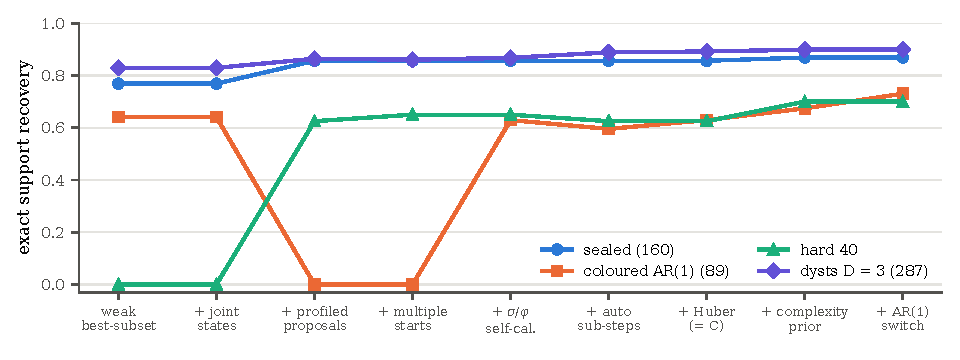
\includegraphics[width=0.92\linewidth]{figures/ablation_ladder.pdf}
\caption{Cumulative ladder from the weak best-subset selector to our method. Up to the last rung the white-noise likelihood is used. Refitting the weak answer jointly (second rung) cannot change its support. The profiled-quadratic proposals give the largest step on white noise, and without self-calibration they overfit every coloured run.}
\label{fig:ladder}
\end{figure}

\paragraph{Subset proposals.} Removing proposals loses 32 exact recoveries and gains none; replacing exhaustive selection with forward stepwise search loses 28 and gains none. On the hard 40, joint refitting of the weak start alone recovers no runs, all starts refitted without proposals recover 19, proposals from the weak start recover 27, and the full method recovers 28. Searching combinations of terms is therefore the principal source of the improvement over refitting existing supports.

\paragraph{Profiling.} A separate prospective ablation builds proposals from $A_{cc}$ and $g_c$, holding the states fixed instead of eliminating their increments. PJSS recovers 490/576 runs versus 480/576 for this variant, with 15 paired wins and 5 losses. On the hard 40 it recovers 28 versus 24; on coloured noise the fixed-state variant has one more recovery. Profiling therefore adds a smaller, setting-dependent gain: it changes how candidates are ranked by accounting for local state adjustment, while both variants retain exhaustive subset proposals and nonlinear joint refits.

\paragraph{Calibration.} Under a white-noise likelihood, proposals overfit every coloured run without noise-scale and penalty calibration; calibration restores recovery in the ladder. Its effect on white noise is negligible. Gaussian loss improves the AR(1) path, motivating the separately confirmed update in \cref{sec:noise}. Other ablations and coefficient errors are reported in \cref{app:ablation-detail}.


\subsection{Comparison with standard baselines}
\label{sec:baselines}

\begin{figure}[t]
\centering
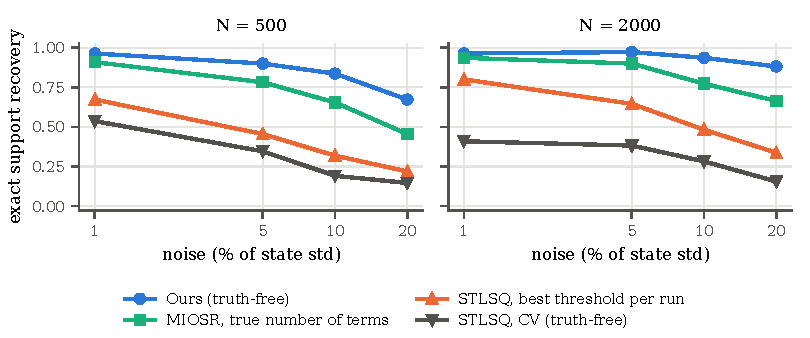
\includegraphics[width=0.82\linewidth]{figures/baselines_noise.pdf}
\caption{Exact recovery on the 880 paired \texttt{dysts} runs, by noise level and record length. Two of the four curves use the truth: STLSQ with the best threshold chosen per run, and MIOSR given the true number of terms in each equation. Each point is the mean of 110 runs.}
\label{fig:baselines-noise}
\end{figure}

PJSS has higher exact recovery than each tested standard baseline on the paired subsets, including the oracle references (\cref{fig:baselines-noise}; all baselines are in \cref{tab:baselines}). The strongest truth-free competitors are SINDy with STLSQ (0.306 against 0.891) and PySR (0.444 against 0.929). The best reference that uses the truth is MIOSR given the true number of terms (0.759), which our truth-free method still beats 123/7. The per-run oracle of the threshold-based baselines is 1.4--2.4 times their best truth-free rule, which confirms that the threshold choice limits them, although it does not explain the whole gap. PySR and ODEFormer are general-purpose methods, and exact recovery is a harsh metric for them. On the hard 40, our method recovers 28 and our Python port of ODR-BINDy, given the true noise level, 14 in its better setting at about 2\,h per run. This comparison concerns the port; equivalence with the original solver has not been validated.

\subsection{Comparison with DEDi}
\label{sec:h2h}
\label{sec:hard}
The closest competitor is the joint-state method DEDi. We pre-registered a comparison on 80 runs, 16 per condition, drawn at random from five archives of the 10 core systems (\cref{tab:dedi}). It therefore covers systems used in development; a second comparison on new systems follows. The hard condition covers Lorenz, Chen and R\"ossler, without Rabinovich--Fabrikant. The primary test is exact recovery against DEDi's default selection by validation error. Secondary analyses are DEDi selecting by BIC, and an oracle that counts a run as exact if any of DEDi's 35 fits is exact, which recovers 64.

\begin{table}[t]
\centering
\caption{Pre-registered comparison with DEDi on 80 random runs: number of runs recovered exactly. \emph{Val} is DEDi's default selection by validation error and \emph{BIC} its alternative. Paired tests are in \cref{tab:h2h}.}
\label{tab:dedi}
\small
\begin{tabular}{@{}lcccc@{}}
\toprule
Condition & $n$ & \textbf{Ours} & DEDi val & DEDi BIC \\
\midrule
Hard (20\%, $N=2000$) & 16 & 15 & 13 & 15 \\
White (10--20\%) & 16 & 14 & 14 & 14 \\
Coloured AR(1) (10--20\%) & 16 & 10 & 5 & 5 \\
Heavy-tailed $t_3$ (10--20\%) & 16 & 14 & 12 & 13 \\
Short ($N=500$, 5--10\%) & 16 & 13 & 11 & 14 \\
\midrule
\textbf{All} & 80 & \textbf{66} & 55 & 61 \\
\bottomrule
\end{tabular}
\end{table}

PJSS recovers 66/80 runs, compared with 55/80 for DEDi's default validation selection and 61/80 for BIC selection. The paired difference for BIC, DEDi minus PJSS, is $-0.062$ (95\% CI $[-0.140,+0.011]$): it meets the pre-specified noninferiority margin of 0.10 but does not establish superiority. Without coloured noise, the two recover the same 56/64 runs. Detailed paired tests and the device sensitivity analysis are in \cref{app:paired}.

A second prospective comparison uses 64 runs of 35 three-dimensional \texttt{dysts} systems outside our development benchmarks. PJSS recovers 53, against 36 with DEDi's validation selection, 41 with BIC and 44 under its oracle (\cref{tab:h2h-dysts}). Resampling systems gives 95\% intervals for the differences of $[-0.413,-0.119]$ and $[-0.344,-0.044]$, respectively; this clustering check was post hoc, with the reproducible resampling procedure in \cref{app:bootstrap}. The advantage is concentrated at 1--5\% noise (29/32 versus 14/32 and 19/32); at 10--20\% noise, PJSS recovers 24/32 versus 22/32 for either selection. These comparisons have different designs and neither covers $D>3$.

\begin{table}[t]
\centering
\caption{Pre-registered comparison of PJSS v1.2 with DEDi on 64 runs of the 35 three-dimensional \texttt{dysts} systems new to us (8 runs per combination of noise and $N$). W/L: runs only ours / only DEDi gets exactly right. The difference is the DEDi exact rate minus ours, with Newcombe's paired 95\% CI. The oracle uses the truth.}
\label{tab:h2h-dysts}
\small
\begin{tabular}{@{}lcccc@{}}
\toprule
Noise & $n$ & \textbf{Ours} & DEDi val & DEDi BIC \\
\midrule
1\% & 16 & 15 & 5 & 8 \\
5\% & 16 & 14 & 9 & 11 \\
10\% & 16 & 14 & 13 & 13 \\
20\% & 16 & 10 & 9 & 9 \\
\midrule
\textbf{All} & 64 & \textbf{53} & 36 & 41 \\
W/L ($p$) & & & 19/2 (0.0002) & 15/3 (0.008) \\
Difference & & & $-0.266$ & $-0.188$ \\
95\% CI & & & $[-0.384,-0.137]$ & $[-0.306,-0.064]$ \\
\midrule
DEDi oracle (uses truth) & 64 & 53 & \multicolumn{2}{c}{44, 12/3 (0.04)} \\
\bottomrule
\end{tabular}
\end{table}

\subsection{Computational cost}
\label{sec:cost}

\begin{figure}[t]
\centering
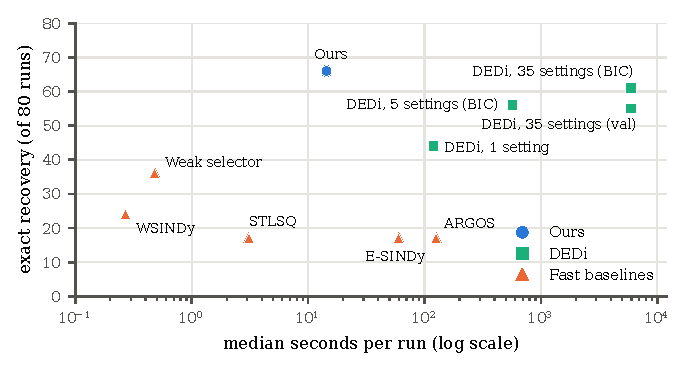
\includegraphics[width=0.66\linewidth]{figures/accuracy_cost.pdf}
\caption{Accuracy against cost on the 80 head-to-head runs. Every method picks its sparsity without the truth. Times are median wall seconds per run on a fully loaded machine. Ours and the fast baselines ran on one CPU core; DEDi ran on a GPU shared by 10 processes for 73 of the 80 runs. Exact values are in \cref{tab:fast}.}
\label{fig:cost}
\end{figure}

\Cref{fig:cost} reports accuracy and wall-clock cost on a loaded NVIDIA GB10 machine; these timings compare execution setups rather than intrinsic costs. A separate measurement on three cases gives about 5\,s per PJSS run. DEDi uses 4{,}374--34{,}006 aggregate single-thread task-seconds across three concurrent CPU workers, or 501--4{,}462\,s with one GPU process. The CPU totals sum elapsed times for 35 grid pairs; they are not measured serial full-grid wall times. Sharing pairs across workers deviated from the prospective CPU protocol; the GPU measurement ran as planned. Two runs are Sprott~A and one is Rabinovich--Fabrikant, which neither method recovers, so these ratios should not be generalised to all systems (\cref{app:timing-detail}).

The computational difference comes from support search. PJSS performs about 21 joint fits and screens candidate subsets cheaply; DEDi performs a backward-elimination sequence for each grid setting. Smaller DEDi budgets reduce cost but also recovery: one setting recovers 44/80 runs, and five settings with BIC recover 56/80. WSINDy is about 50 times faster than PJSS on the loaded-machine comparison and recovers 24/80. Scaling results are in \cref{app:more}.

\subsection{Coloured noise}
\label{sec:noise}
Coloured AR(1) noise is the hardest setting, because slow noise excursions resemble dynamics. The base model gains only 3 points over the weak selector (0.674 against 0.645), and the AR(1) likelihood with the automatic switch raises this to 0.761. The switch fired on 100\% of coloured test runs and on 0\% of sealed and confirmation runs. The ablation then showed that Huber loss hurts inside the AR(1) likelihood (\cref{sec:ablation}). That finding came from a test subsample, so we redeveloped the change on development data and pre-registered a fresh coloured archive of 800 runs, on which the Gaussian loss raises exact recovery from 0.754 to 0.805 (43 paired wins, 2 losses). It changed 0 of 1{,}600 answers on the white and $t_3$ archives.

\subsection{Real data}
\label{sec:realdata}
Our real-data tests are negative or anecdotal.

\paragraph{Lynx and hare.} On the 21 annual Hudson's Bay pelt counts, a standard example that E-SINDy~\citep{fasel2022esindy} solves, the model returns a degenerate answer whose integration diverges, and it does not flag it. These data are far below the $N=500$--2{,}000 regime the method was built for. On a cubic-spline resampling (201 points) it finds all four Lotka--Volterra terms plus one weak extra term, but the method was never validated on interpolated data, so this is an anecdote.
% Source: docs/reports/real_data.md; results_real/lynx_hare.json, results_real/lynx_hare_v101.json.

\paragraph{Measured pendulums.} We found no public recording of a chaotic system whose accepted model is polynomial, so we used the multi-arm pendulum rig of \citet{kaheman2023pendulum} with a pre-registered protocol. For the single pendulum, the coordinates $(\sin\theta,\cos\theta,\dot\theta)$ put the accepted model $\ddot\theta=A\sin\theta-B\dot\theta$ in the library. The method fails the pre-specified support criterion. It finds the gravity term ($A$ within 0.2\%) and both kinematic terms, but it drops the damping term and adds 11 small terms, which stand in for dissipation. No pysindy baseline has the exact support anywhere on its threshold path. However, $\sin^2\theta+\cos^2\theta=1$ and its multiples make the cubic library dependent on this embedding manifold. Distinct supports can represent the same dynamics there, so failure to recover the selected support alone does not establish dynamical failure; an equivalence-aware evaluation was not performed.

The double pendulum's accepted model is rational in $\cos(\theta_1-\theta_2)$, so it lies outside every library we have, and our method is worse than the pysindy baselines: its forecast stays valid for 0.024--0.127\,s, against 0.47--1.47\,s for SINDy and about 0.13\,s for persistence. It never recovers the identities $\dot\theta_i=\omega_i$, which the equation-wise baselines find almost exactly, and it does not flag the answer. Our hypothesis, not tested further, is that when some equations cannot be represented, the joint objective distorts the ones that can, whereas equation-wise regression keeps a misspecified equation from contaminating the others.
% Source: docs/reports/real_data2.md; results_real2/{single,double}_*.json, results_real2/tables.md.
% Pre-registration: results_real2/PREREGISTRATION.md; data sources and sha256: results_real2/SOURCES.md.
